\documentclass[bachelor, och, labwork]{shiza}

\usepackage[utf8]{inputenc}
\usepackage{graphicx}

\usepackage[sort,compress]{cite}
\usepackage{amsmath}
\usepackage{amssymb}
\usepackage{amsthm}
\usepackage{fancyvrb}
\usepackage{longtable}
\usepackage{array}
\usepackage[english,russian]{babel}
\usepackage{minted}

\usepackage{tempora}


% \usepackage[colorlinks=false]{hyperref}


\newcommand{\eqdef}{\stackrel {\rm def}{=}}


\begin{document}

\title{Алгоритмы алгебры и теории чисел}

\course{4}

\group{431}

\napravlenie{10.05.01 "--- Компьютерная безопасность}


\author{Никитина Арсения Владимировича}


\satitle{доцент}
\saname{А.\,С.\,Гераськин}


\date{2022}

\maketitle

% Включение нумерации рисунков, формул и таблиц по разделам
% (по умолчанию - нумерация сквозная)
% (допускается оба вида нумерации)
%\secNumbering


\tableofcontents

\section{Задание лабораторной работы}

Осуществить факторизацию с помощью алгоритма Диксона.

\section{Теоретическая часть}

Алгоритм Диксона факторизации чисел использует в своей основе идею Лежандра,
заключающуюся в поиске пары целых чисел $x$ и $y$ таких, что:

$$x^2 \equiv y^2 \pmod n, ~ x \not\equiv \pm y \pmod n$$.

\begin{center}
    \textit{Описание алгоритма}
\end{center}

\begin{enumerate}
    \item Составить факторную базу $B = \left\{ {p_1,p_2,\dots,p_h} \right\}$, 
    состоящую из всех простых чисел $p \leq M = L\left({n}\right)^\frac{1}{2}$, 
    где $L\left({n}\right)=\exp\left({\sqrt{\ln{n}\cdot \ln{\ln{n}}}}\right)$.
    \item Выбрать случайное $b, \sqrt{n}<b<n$.
    \item Вычислить $a = b^2\bmod{n}$.
    \item Проверить число $a$ на гладкость пробными делениями. Если $a$ является
    $B$-гладким числом, то есть $a = \prod_{p\in B}p^{\alpha_{p}\left({b}\right)}$,
    следует запомнить вектора $\vec{\alpha}\left({b}\right)$ и $\vec{\varepsilon}\left({b}\right)$:
        \begin{enumerate}
            \item $\vec{\alpha}\left({b}\right)=\left({\alpha_{p_1}\left({b}\right), \dots, \alpha_{p_h}\left({b}\right)}\right)$,
            \item $\vec{\varepsilon}\left({b}\right)=\left({\alpha_{p_1}\left({b}\right)\bmod{2}, \dots, \alpha_{p_h}\left({b}\right)\bmod{2}}\right)$.
        \end{enumerate}
    \item Повторять процедуру генерации чисел $b$ до тех пор, пока не будет 
    найдено $h+1$ $B$-гладких чисел $b_1,...,b_{h+1}$.
    \item Методом Гаусса найти линейную зависимость среди \\векторов
    $\vec{\varepsilon}\left({b_1}\right), \dots, \vec{\varepsilon}\left({b_{h+1}}\right)$:
    \begin{center}
        $\vec{\varepsilon}\left({b_{i_1}}\right)\oplus\dots\oplus\vec{\varepsilon}\left({b_{i_t}}\right)=\vec{0}, ~t=\overline{1,m}$.
    \end{center}
    \item Положить $x=b_{i_1} \dots b_{i_t}\bmod{n}$ и $y=\prod_{p\in B}p^{\left({ \alpha_p\left({b_{i_1}}\right)+\dots+\alpha_p\left({b_{i_t}}\right) }\right) \over{2}}\bmod{n}$.
    \item Проверить $x \equiv \pm y \pmod{n}$. Если это так, то повторить
    процедуру генерации. Если нет, то найдена нетривиальное разложение:
    \begin{center}
        ${\displaystyle n=u\cdot v,u=gcd\left({x+y,n}\right),v=gcd\left({x-y,n}\right).}$
    \end{center}
\end{enumerate}


\section{Практическая часть}
\subsection{Пример работы алгоритма}
\begin{figure}[H]
    \centering
    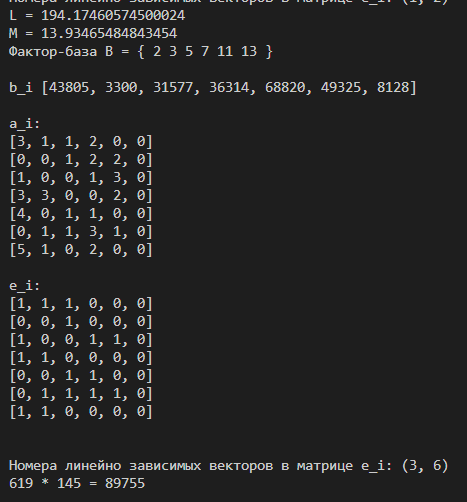
\includegraphics[width=1\textwidth]{pic1.png}
    \caption{}
\end{figure}

\setminted[python]{linenos,breaklines=true, fontsize=\small, style=bw}
    \subsection{Код программы, реализующей рассмотренный алгоритм}
        \inputminted{python}{lab12.py}


\end{document}